\begin{itemize}
 \item Forward / backward formulation
 \item Padding
\end{itemize}


\paragraph{Padding. }

\begin{figure}
 \begin{center}
  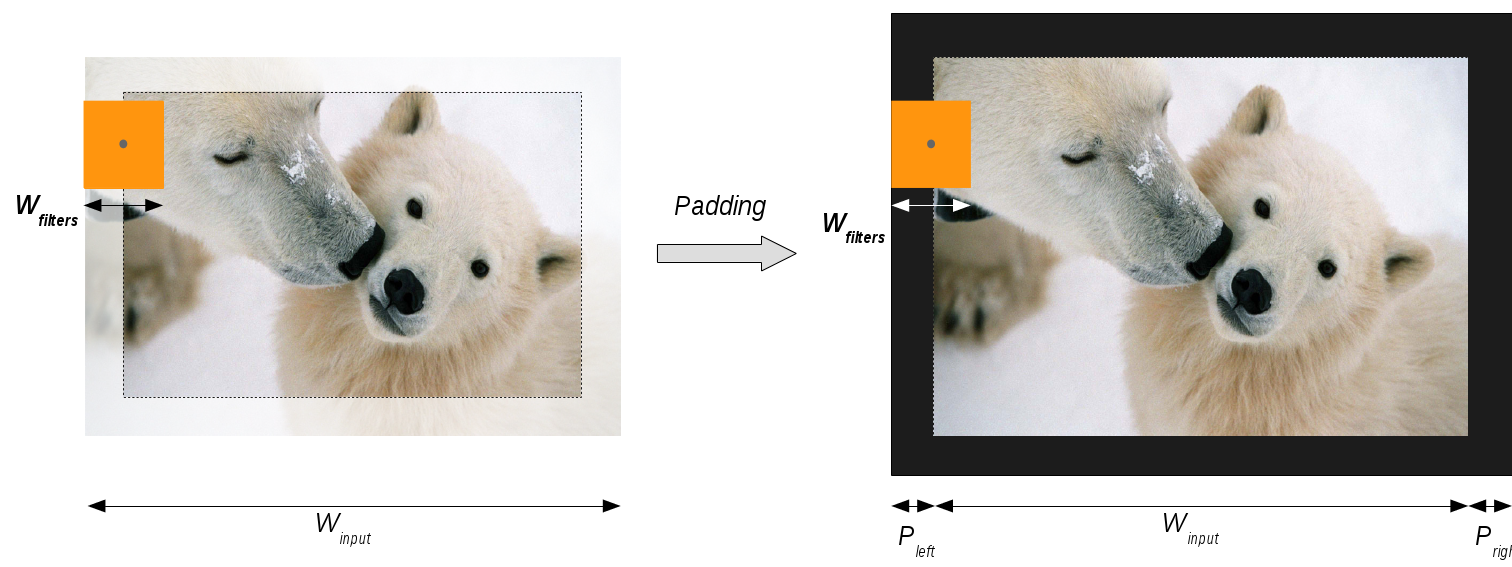
\includegraphics[width=16cm]{images/padding.png}
 \end{center}
  \caption{
  \label{fig:padding}
  Padding. Due to the filters width, the filters cannot be applied to the borders of the image. Padding consists in enlarging the 
  image by zeros, which enables the filters to be applied to the \textit{entire} image (including borders). 
  }
\end{figure}

In figure \ref{fig:padding}, we represent the padding (or ``zero-padding'') process. It consists in artificially augmenting the size of the input 
image (or map) in order to avoid border effects. Indeed, due to the width of the convolutional filters applied to the input maps, the center of the 
filters (represented as the grey dot in figure \ref{fig:padding}) cannot be at the border of the image.
The total number of possible positions for the center of the filters is: 
\begin{align}
 W_{input} - W_{filters} + 1 \nonumber
\end{align}

However, if zeros are added at the border of the image, the center of the filters can be positionned at the border of the input image, so that the 
filters do not suffer from border effects. 
The total number of positions for the center of the filters is then: 
\begin{align}
 \underbrace{W_{input} + P_{left} + P_{right}}_{\textit{zero-padded image}} - W_{filters} + 1 \nonumber
\end{align}

Obviously, this process is applied in the same fashion no matter if the input is a set of maps or an 
image.




\paragraph{Convolutions. }

\begin{figure}
 \begin{center}
  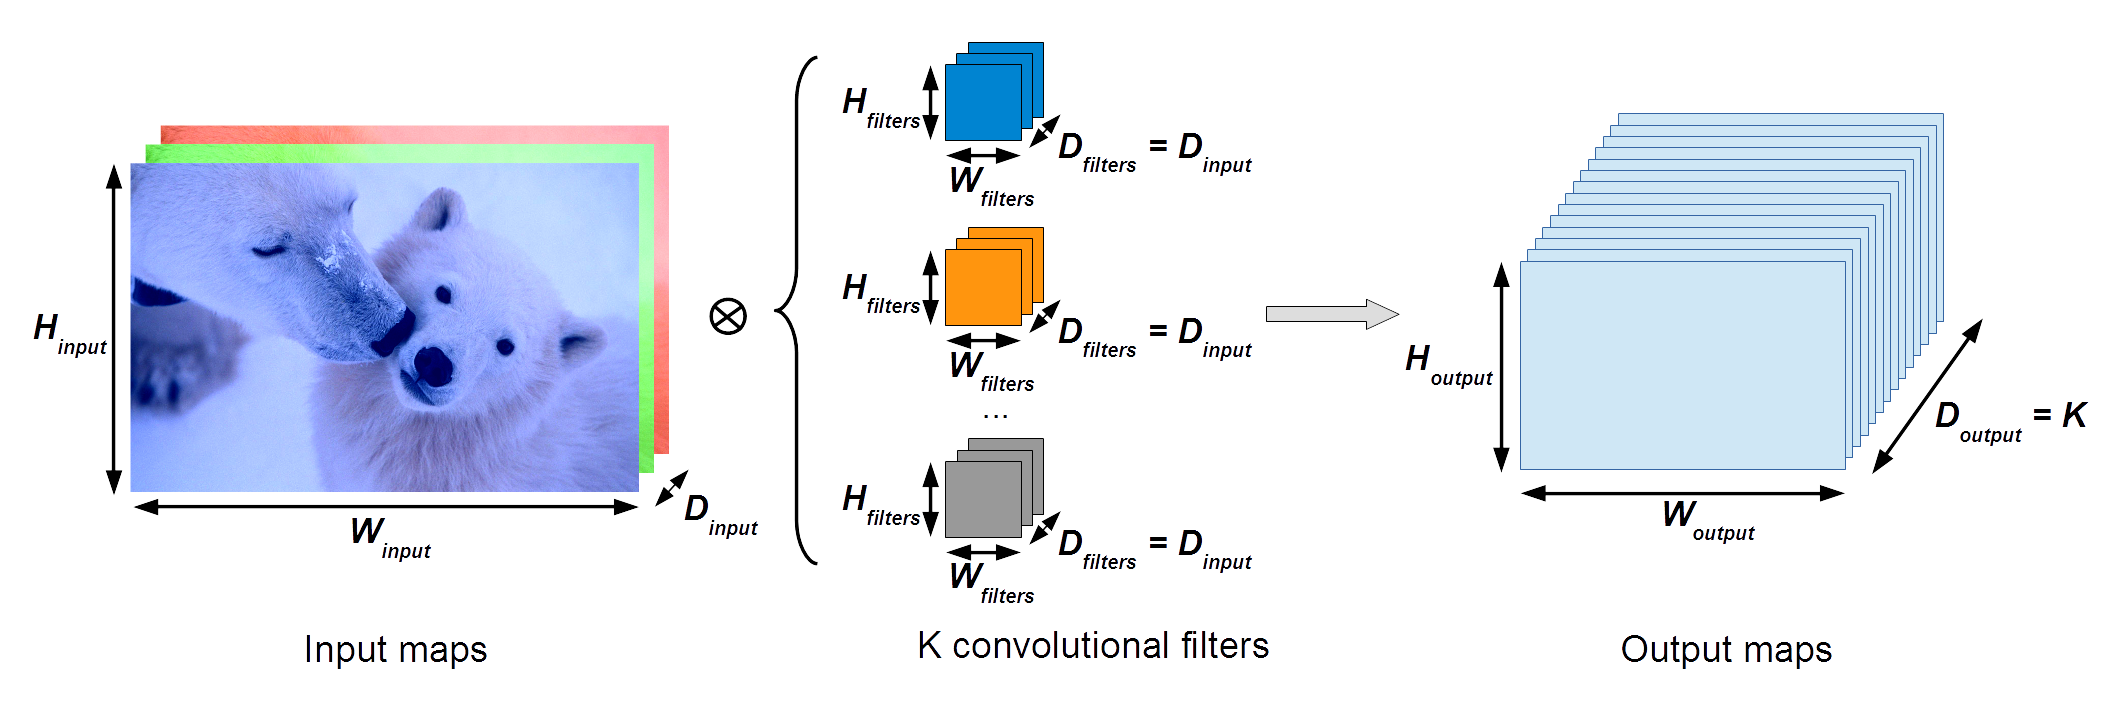
\includegraphics[width=16cm]{images/schema_conv.png}
 \end{center}
  \caption{
  \label{fig:conv}Convolution scheme. 
  }
\end{figure}

In figure \ref{fig:conv}, we represent the general scheme for convolution. 
The width of the ouput map is: 
\begin{align}
 W_{output} = \lfloor \frac{W_{input} + P_{left} + P_{right} - W_{filters}}{\delta_{filters}} \rfloor + 1 \nonumber
\end{align}
A equation can be written for the height of the output map. 

The depth of the output map is however equivalent to the number of filters. Indeed, one map is produced for each of the $K$ filter banks; 
these response maps are then stocked as a 3D matrix. 

